\section{Drift Chamber Electronics}
\subsubsection{On-Chamber PCBs and Cables}
After the drift chambers were built and the wires strung, we mounted
on-chamber printed circuit boards onto the chamber endplates.
The signal connections to the wires are made through printed-circuit 
boards mounted along one side of each chamber, called Signal Translator 
Boards (STBs).  These boards are responsible for signal routing and 
pre-amplification.  

On the opposite side of each sector, another set of 
circuit boards called the High Voltage Translator Boards (HVTBs) is used 
to make the high-voltage connections to the wires (see the subsection
on gas, low voltage and high voltage for more details on the high
voltage system).

The drift chamber signal amplification and readout consists of the 
following subsystems:
\begin{itemize}
\item  chamber-mounted printed circuit boards with a single in-line package
(SIP) amplifier for each signal wire; these are the STB's
\item  chamber printed circuit boards which distribute high voltage
to all of the wires; these are the HVTB's
\item a single 17-pair twisted-pair readout cable for each group of 16
SIP's, and
\item a 96-channel drift chamber readout board (DCRB) for each group
of 6 cables (96 signal wires)
\end{itemize}


%%%%%%%%%%%%%%%%%%%%%%%%%%%%%%%%%%%%%%%%%%%%%%%%%%%%%%%%%%%%%%%%%%%%%%%%%
\begin{table}[htbp]
\begin{center}
\begin{tabular} {||c|c||} \hline \hline
{\bf Component}           & {\bf Number} \\ \hline
STB boards (6 types)      & 252 total \\ \hline
HVTB boards (6 types)     & 252 total \\ \hline
low-voltage cables        & 252 total  \\ \hline
high-voltage cables       & 252 total  \\ \hline
signal cables (17-pair)   & 1512 \\ \hline
total signals             & 24192 \\ \hline \hline
\end{tabular}
\caption{\small{Electronic channel counts for the readout, high voltage,
and low voltage.}}
\label{electronic-channels}
\end{center}
\end{table}
%%%%%%%%%%%%%%%%%%%%%%%%%%%%%%%%%%%%%%%%%%%%%%%%%%%%%%%%%%%%%%%%%%%%%%%%%



The circuit boards that interface the sense 
wires to the pre-amplifiers (STBs) were  
designed for a 96-channel format.  This format requires seven 
circuit boards for each superlayer (672 signals).   


Fig.~\ref{trace-routing-schematic} shows the traces 
routed from the signal pick-up at the plated-through holes to the signal 
inputs of the pre-amplifier.

%%%%%%%%%%%%%%%%%%%%%%%%%%%%%%%%%%%%%%%%%%%%%%%%%%%%%%%%%%%%%%%%%%%%%%%%%%%
\begin{figure}[htbp]
\vspace{5cm}
\begin{picture}(50,50)
\put(-10,10)
{\hbox{\includegraphics[width=0.35\textwidth,natwidth=610,natheight=642]{img/trace-routing-schematic.jpg}}}
\end{picture}
\caption{\small{Trace routing shown on one of the Region~1 STBs being
designed.}}
\label{trace-routing-schematic}
\end{figure}
%%%%%%%%%%%%%%%%%%%%%%%%%%%%%%%%%%%%%%%%%%%%%%%%%%%%%%%%%%%%%%%%%%%%%%%%%%%

The heart of the STB board is an individually packaged
single in-line package (SIP) preamplifer which was modified
from the design of the previous CLAS detectors and 
included an epoxy resin encapsulation.  
The encapsulation of the components was included to prevent 
component corrosion in a somewhat humid environment (relative
humidities as high as 60\%).
These ``CP01'' pre-amplifiers provide the gain, dynamic range, rise time, low 
noise, and low power needed for the performance requirements.  The CP01 is
a transimpedance amplifier with a gain of $2 mV/\mu Amp$ and a rise-time
less than $10 ns$.  Each SIP operates at 6V and draws about $13 mA$.   

Fig.~\ref{CP01-description} shows the design and specifications of the
CP01 pre-amplifier.

%%%%%%%%%%%%%%%%%%%%%%%%%%%%%%%%%%%%%%%%%%%%%%%%%%%%%%%%%%%%%%%%%%%%%%%%%%%
\begin{figure}[htbp]
\vspace{5cm}
\begin{picture}(50,50)
\put(10,-10)
{\hbox{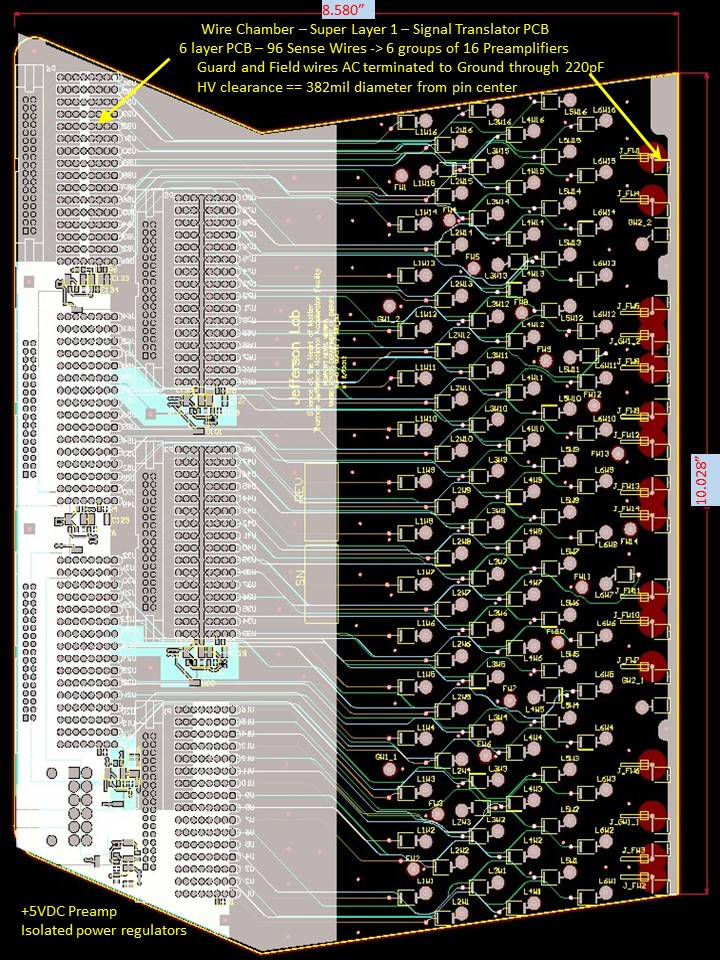
\includegraphics[width=0.35\textwidth,natwidth=610,natheight=64]{img/CP01-description.jpg}}}
\end{picture}
\caption{\small{The CP01 pre-amplifier design and specifications.}}
\label{CP01-description}
\end{figure}
%%%%%%%%%%%%%%%%%%%%%%%%%%%%%%%%%%%%%%%%%%%%%%%%%%%%%%%%%%%%%%%%%%%%%%%%%%%

Each group of 16 pre-amplifier output signals were routed to a 17 pair connector.
Sixteen of the pairs are used as differential signal paths which are routed from the STB's to the 
drift chamber readout boards (DCRB) over individual cables consisting of 16 twisted pairs.  
The seventeenth pair is used to send a calibration pulse from the DCRB
to the STB preamplifier group. We chose
twisted-pair readout because of its immunity to electronic noise.
The cables are round-jacketed with a 
0.025-in pitch so that the overall cable dimension is smaller than the 
standard 17-pair cable.  
 


\subsubsection{Mounting Electronics Boards onto the Chamber}

The signal side of each chamber was tiled with multi-layered printed circuit 
boards called Signal Translation Boards (STBs).  These boards were designed 
to capacitively decouple high voltage from the signals, and then to route 
the signals to the single in-line package (SIP) transimpedance pre-amplifiers 
mounted on these boards.  The amplified differential signals are then sent 
via 20-m long twisted-pair lines to the main {\tt CLAS12} readout electronics.

The connections between the sense-wire crimp pins and the plated-through holes 
of the STB boards were made using short conductive-rubber tubes.  This material 
consists of silver-plated and/or nickel-plated glass spheres embedded in a 
silicon-rubber matrix.  These tubes pass through the plated-through hole and 
over the end of the crimp pins, making the electrical contract between the 
wire and the circuit board.  A small plastic cap inserted into the end of the 
tube ensures good contact with the circuit board.  This approach has the 
advantages of reducing the space needed for connections, preventing crimp pins 
from being pulled from the feedthroughs when disconnecting the boards from the 
wires, and reducing the cost compared to metal connectors.  This detail is 
shown in Fig.~\ref{wire-to-amplifier}.

%%%%%%%%%%%%%%%%%%%%%%%%%%%%%%%%%%%%%%%%%%%%%%%%%%%%%%%%%%%%%%%%%%%%%%%%%%%
\begin{figure}[htbp]
\vspace{5cm}
\begin{picture}(50,50)
\put(20,20)
{\hbox{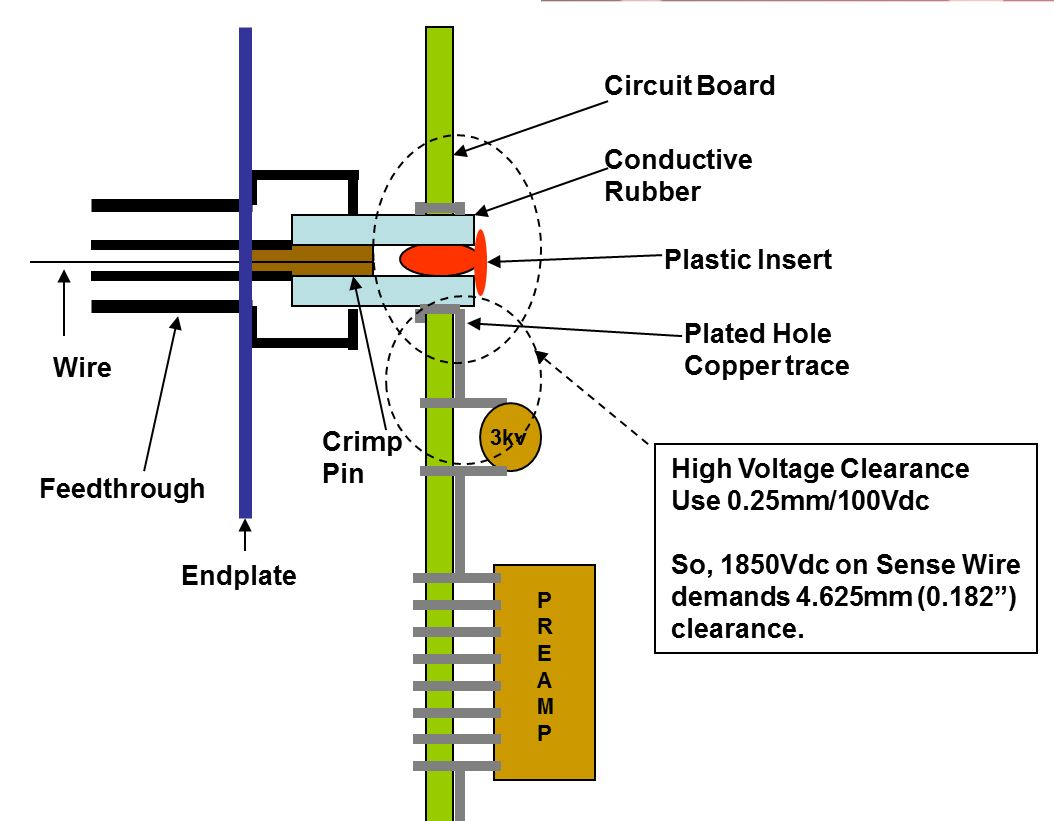
\includegraphics[width=0.7\textwidth,natwidth=610,natheight=642]{img/wire-to-amplifier.jpg}}}
\end{picture}
\caption{\small{ An assembly drawing showing how the crimp pin was inserted
into the feedthrough and how the conductive elastomer tube fits over the 
crimp pin and inside the plated-through hole on the printed circuit board to 
make the electrical connection. Also shown is the signal path from the wire's
crimp pin to the pre-amplifier.  }}
\label{wire-to-amplifier}
\end{figure}
%%%%%%%%%%%%%%%%%%%%%%%%%%%%%%%%%%%%%%%%%%%%%%%%%%%%%%%%%%%%%%%%%%%%%%%%%%%


\subsection{Off-Chamber Amplification, Time Digitization and Readout}

Our on-chamber 
pre-amplifiers send signals to the readout boards (DCRB) 
which provide another level of amplification, 
signal discrimination, adjustable threshold setting, time digitization
and readout. 

These DCRB's are based on FPGA technology, and in addition to
their primary function of amplification, discrimination, digitization
and readout, they are used in a simple ``cluster-finding'' algorithm
to find track segment candidates with a latency of only hundreds
of nanoseconds.

\subsubsection{Drift Chamber Readout Boards (DCRB)}

The DCRB is a 96 channel board that is a combination post-amplifier,
discriminator, time-to-digital converter (TDC) and also has a trigger
output path to provide track segment information for an online tracking trigger.
Fourteen such boards are housed in
a proprietary 9U, 160 mm depth, VXS form factor/crate.
The whole system consisted of 18 such crates, one for each drift chamber.

To perform its time digitization task, the DCRButilizes on-board synchronization to
return the signal time relative to an input time signal from  a Trigger Distribution
Crate.
Its design and architecture
allows it to achieve the following performance metrics:
\begin{itemize}
\item DCRB Performance Metrics
\begin{itemize}
\item Amplification: variable gain from X10 to X30 eliminates saturation
\item Time Digitization: accuracy better than 1 ns; exceeds DC specifications
\item Whole Crate Time Synchronization: through backplane; eliminates cables
\item Event Buffer Size: 500,000 signals
\item VME Transfer Rate: 200 MB/sec
\item Maximum Trigger Rate: greater than 1 MHz
\item Dead-time: 32 ns
\item Scaler: 1 32 bit scaler per channel
\item Track Segment Finding: employs segment-hit dictionary in 32 ns bins
\item Track Segment Reporting: reports found segments to the next-level Track Finder
\end{itemize}
\end{itemize}

In addition to its primary functions of time digitization of DC signals and online
track-finding, the internal scaler functions allow the DCRB to be used in 
a stand-alone manner to efficiently monitor chamber operation during commissioning
and testing.

